% Ch. 1, Fig. 1.1: the setting of the thesis in plain words (no notation; Ch. 1 defines none).
% Images: scripts/make_diagram_assets.py (example volumes of fig:ch4_examples, reference masks only,
% no predictions). Task order and text prompts: original order, thesis/data_description.tex (Sec. 4.2) and thesis/experiment_results.tex.
% DSC of the pretrained model: thesis/tables/cl_metrics.csv, row "Pretrained model (Task Order=Original)":
%   control_pretrained 0.979 (lung, AeroPath test split); adaptation 0.114 (mean over the six knee tasks,
%   SKM-TEA test split; for the never-updated model this is its mean DSC on the knee structures).
% Build: python scripts/build_tikz.py
%
% PLAN
% Card row (images on one baseline): I0 at the origin; I1, I2 right of it; dots node D; I6.
%   Each card Cj = fit around title Tj (above Ij), image Ij, text Pj (below Ij, two lines).
%   P0 holds the DSC of the pretrained model, P1..P6 the text prompts.
%   Connections (straight, horizontal at the image row, east -> west): C0->C1, C1->C2, C2->D, D->C6.
% Brace above C1..C6 (north west of C1 to north east of C6), label above it.
% Brace below C0..C6 (south east of C6 to south west of C0, so it opens upwards), label below it.
\documentclass[12pt,tikz,border=2pt]{standalone}
% Shared preamble of the standalone TikZ figures: same engine, class size, fonts and
% math packages as thesis_main.tex (pdfLaTeX, 12 pt, T1 + Latin Modern, amsmath, bm).
\usepackage[utf8]{inputenc}
\usepackage[T1]{fontenc}
\usepackage{lmodern}
\usepackage{amsmath,amssymb,bm}
\usepackage{graphicx}
\usepackage{xcolor}
\usetikzlibrary{arrows.meta, positioning, calc, fit, backgrounds, decorations.pathreplacing}
\pgfdeclarelayer{panel}            % below the background layer: large panel frames
\pgfsetlayers{panel,background,main}
\def\mat#1{\ensuremath{\bm#1}}   % as lmedoc/math.sty
\def\vec#1{\ensuremath{\bm#1}}
% Colours: base colours of the VoxTell sketch, one colour per strategy component
\definecolor{voxorange}{HTML}{F2A65A}
\definecolor{voxblue}{HTML}{6CA6E0}
\definecolor{voxgreen}{HTML}{8DBF8B}
\definecolor{voxyellow}{HTML}{F5D76E}
\definecolor{voxred}{HTML}{E8877F}
\definecolor{voxlora}{HTML}{D1495B}
\definecolor{voxprompt}{HTML}{7A4FC9}
\definecolor{voxmeta}{HTML}{1B8A8F}
\definecolor{voxkd}{HTML}{C2308F}
\tikzset{lock/.pic={
  \draw[line width=0.6pt] (-0.07,0.02) -- (-0.07,0.09) arc[start angle=180, end angle=0, radius=0.07] -- (0.07,0.02);
  \fill[black!70] (-0.1,-0.1) rectangle (0.1,0.03);
}}
\newif\ifvoximpl     % VoxTell as used (stage-4 keys/values) instead of as in the paper (bottleneck)
\newif\ifvoxannotate
\newif\ifvoxpanel

\begin{document}
\begin{tikzpicture}[
    font=\footnotesize,
    img/.style={inner sep=0pt, outer sep=0pt},
    ttl/.style={inner sep=0.5mm, text height=1.6ex, text depth=0.4ex},
    prm/.style={inner sep=0.5mm, align=center, text width=\imgw, text height=1.6ex},
    card/.style={draw=black!70, line width=0.5pt, rounded corners=1pt, inner sep=1.2mm},
    flow/.style={-{Stealth[length=2mm]}, line width=0.5pt, black!70},
    brc/.style={decorate, decoration={brace, amplitude=1.5mm}, line width=0.5pt, black!70},
  ]
\def\imgw{28.5mm}
\def\cgap{10.5mm}   % between images of neighbouring cards (card padding + arrow)

% Card row
\node[img] (I0) {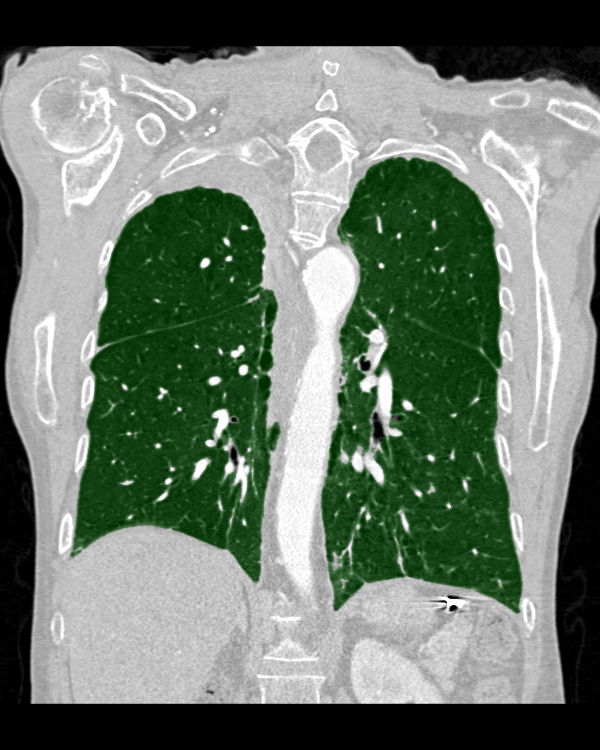
\includegraphics[width=\imgw]{ch1_lung.png}};
\node[img, right=\cgap of I0] (I1) {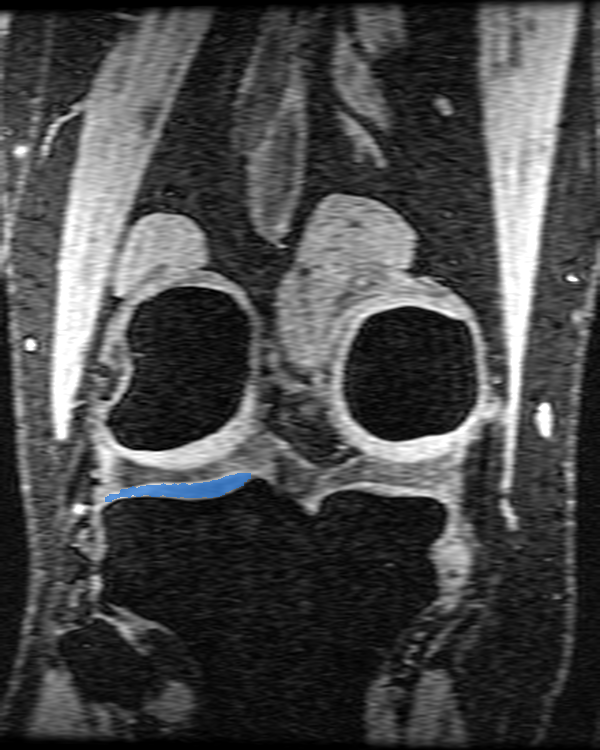
\includegraphics[width=\imgw]{ch1_task_lateral_tibial.png}};
\node[img, right=\cgap of I1] (I2) {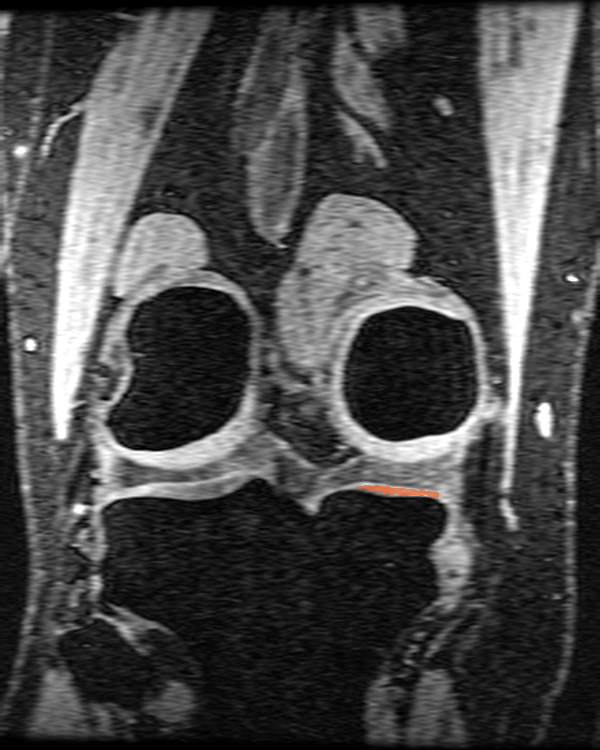
\includegraphics[width=\imgw]{ch1_task_medial_tibial.png}};
\node[right=7.5mm of I2, inner sep=0.5mm] (D) {\dots};
\node[img, right=7.5mm of D] (I6) {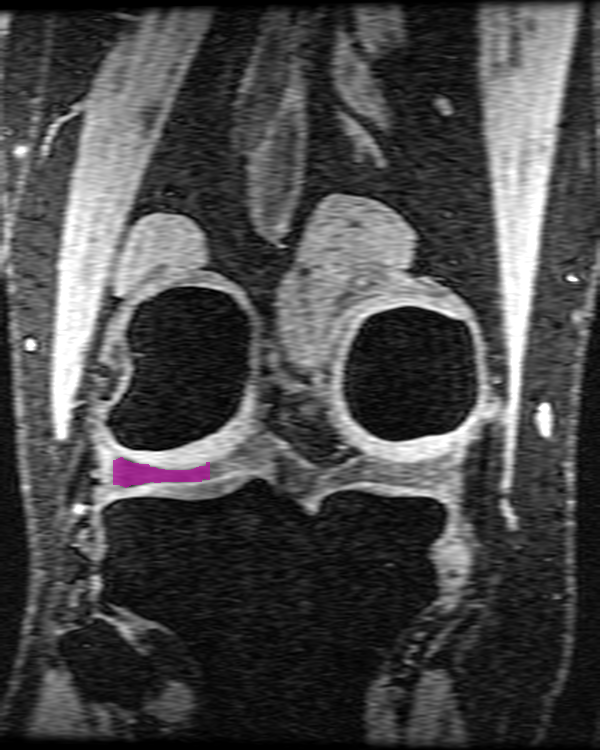
\includegraphics[width=\imgw]{ch1_task_lateral_meniscus.png}};
\foreach \j/\t/\p in {0/pretrained VoxTell/{lung: DSC 0.979\\knee: DSC 0.114},
                      1/task 1/{``lateral tibial\\cartilage''},
                      2/task 2/{``medial tibial\\cartilage''},
                      6/task 6/{``lateral\\meniscus''}} {
  \node[ttl, above=0.8mm of I\j] (T\j) {\t};
  \node[prm, below=0.8mm of I\j] (P\j) {\strut\p\strut};   % struts: equal height of all texts
  \node[card, fit=(T\j)(I\j)(P\j)] (C\j) {};
}
% horizontal at the height of the images (all images share one baseline)
\draw[flow] (C0.east |- I0) -- (C1.west |- I1);
\draw[flow] (C1.east |- I1) -- (C2.west |- I2);
\draw[flow] (C2.east |- D) -- (D.west);
\draw[flow] (D.east) -- (C6.west |- D);

% Brace over the tasks
\draw[brc] ([yshift=1.5mm]C1.north west) -- ([yshift=1.5mm]C6.north east)
  node[midway, above=2mm, inner sep=0.5mm] {new structures, one after another, few labelled volumes each};

% Brace under all cards
\draw[brc] ([yshift=-1.5mm]C6.south east) -- ([yshift=-1.5mm]C0.south west)
  node[midway, below=2mm, inner sep=0.5mm] {after every task, the same model has to segment all of these};
\end{tikzpicture}
\end{document}
